%!TEX root = ../report.tex


\chapter{Project Management}\label{ch:project-management}


\section{Project Charter}\label{sec:project-charter}

\begin{table}[htp]
    \centering
    \caption{Project Charter General Details}
    \begin{tabular}{@{}|l|l|@{}}
        \toprule
        \textbf{Activity} & \textbf{Date} \\
        \midrule
        Project Name & Trale / SocialStuff (former working title) \\
        \midrule
        Submitted by \& date & Dave Hoevenaars, Maurits van der Zee, 28-09-2020 \\
        \midrule
        Strategic Objective &
        \parbox[t]{8cm}{Providing a decentralized, privacy focussed messenger as competitor to currently present centralized alternatives.} \\
        \midrule
        Project ID & SOFA2020-HOM02-SocialStuff \\
        \midrule
        Confidentiality & N/A \\
        \bottomrule
    \end{tabular}
    \label{tab:my-table}
\end{table}

\subsection{Problem Statement}\label{subsec:problem-statement}

Centralized social media platforms have been dominating the market for the last decade.
This is a problem because nearly everybody who is communicating throughout the internet is relaying on those businesses,
who's business model involves selling your private data.
This can be especially damaging for high-profile individuals which need to stay private or celebrities who want to keep
up reputation and credibility.
Additionally, the large corporations that host such services are based in countries which can force those businesses to
provide access to their systems (e.g.\ USA, China \& Russia).

\subsection{Objective}\label{subsec:objective}

The goal of the Trale project sequence is to develop a working prototype of the decentralized chat application
(frontend \& backend) as well as supporting documentation.
This will be done by January 8th, 2021.

\subsection{Critical Success Factors}\label{subsec:critical-success-factors}

In order to prove Trale's claim of privacy and security, a penetration test should be carried out, and the
results should be divided in five sub-sections: Reconnaissance, Scanning, Gaining Access, Maintaining Access, and
Covering tracks.
In these categories a risk analysis will be carried out and if the exposure is not greater than two, the penetration
test will be considered as a pass.

\subsection{Risks}\label{subsec:risks}

In the Trale project we identified a few risks which may occur such as:

\begin{itemize}
    \setlength\itemsep{-0.5em}
    \item Not achieving customer satisfaction due to not meeting the client's requirements
    \item Employee capacity decrease because of illness
    \item Stretching the project's time scope due to unfamiliarity with programming languages and/or technologies
\end{itemize}

\subsection{Scope focus}\label{subsec:scope-focus}

In scope of the Trale project sequence is:
creation of a prototype of a decentralized chat application.

\begin{itemize}
    \setlength\itemsep{-0.5em}
    \item A report explaining analysis, design and implementation choices
    \item Creation of frontend, backend, and libraries of Trale
    \item Analysis, Design and in-code documentation artifacts
    \item Optional: Customer Website
\end{itemize}

However, in this project sequence we will not have a fully released version of Trale Messenger, and the chat application
will not be deployed either.
The main goal is to have a working prototype, in order to showcase the potential of the project.

\subsection{Key activities \& dates}\label{subsec:key-activities-and-dates}

\begin{table}[H]
    \centering
    \begin{tabular}{@{}|l|l|@{}}
        \toprule
        \textbf{Activity}       & \textbf{Date} \\
        \midrule
        Project Kick-off        & 09/02/2020     \\
        \midrule
        Business case           & 10/01/2020    \\
        \midrule
        Project Management Plan & 10/01/2020    \\
        \midrule
        Project Charter         & 10/15/2020    \\
        \midrule
        Project Scope Baseline  & 10/25/2020    \\
        \midrule
        WBS                     & 10/30/2020    \\
        \midrule
        Project Poster          & 01/06/2021    \\
        \midrule
        Project Handover        & 01/20/2021    \\
        \bottomrule
    \end{tabular}
    \label{tab:table2}
\end{table}

\subsection{Deliverables}\label{subsec:deliverables}

\begin{itemize}
    \setlength\itemsep{-0.5em}
    \item Creation of prototype of Trale Messenger
    \item A report explaining analysis, design and implementation choices
    \item Creation of frontend of Social Stuff
    \item Creation of backend of Social Stuff
    \item Analysis, Design and in-code documentation artefacts
    \item Optional: Customer Website
\end{itemize}

\subsection{Business Case}\label{subsec:business-case}

The business case in non-financial;
providing customer satisfaction by delivering a social media platform which is excellent in its privacy standards.

\subsection{Proposed start \& end dates}\label{subsec:proposed-start-and-end-dates}

The Trale project will start at \textbf{09/02/2020} and will end \textbf{01/08/2021}.

\subsection{Stakeholders \& Resources}\label{subsec:stakeholders-and-resources}

The resources we will utilize for the completion of the Trale project includes:
\begin{itemize}
    \setlength\itemsep{-0.5em}
    \item Trello, for a Kanban style agile project management
    \item A shared repository on GitHub to do work simultaneously
    \item MS Teams platform for general communication and team meetings
    \item Adobe XD for \ac{ux} and \ac{ui} design
    \item Coding standards
    \item The source Code
    \item Open source libraries
\end{itemize}

Furthermore, to support the completion of the project the following stakeholders are involved:
\begin{itemize}
    \setlength\itemsep{-0.5em}
    \item Gerhard Bongardt: Business Owner
    \item Pieter van den Hombergh: Project Governance
    \item Malte Castner
    \item Dave Hoevenaars
    \item Tobias Jansen
    \item J\"orn Neumeyer: Product Owner, Backend architect
    \item Klaas Maurits van der Zee: Project Manager, Frontend developer
\end{itemize}

\section{Project Management Plan}\label{sec:project-management-plan}

\subsection{Management Summary}\label{subsec:management-summary}

The joint collaboration between: Gedak GmbH, Trale and the \ac{sofa} Fontys students is resulting in to a project
sequence.
The final goal is to provide an implementation of an encrypted chat platform which enables users to stay private by
establishing a decentralized structure in which pseudo anonymity can be guaranteed.
The project is mainly focused on providing a working prototype and providing thorough documentation.
The project's scope and justification will be discussed in this document.

\subsection{Introduction}\label{subsec:introduction}
This document will provide an overview over the Trale project.
To achieve this, the project will be briefly explained, what the final products will be and who the stakeholders are.
Afterwards the document will address, which potential risks could occur during the development and how the team will
mitigate with them.
Next it will be addressed, how the change management will be handled during development and how a high quality can be
ensured.
Finally, the communication plan will be introduced.

\subsection{Trale}\label{subsec:trale}

This chapter explains the company briefly;
it also describes the problem description and our tasks within the duration of the project.

\subsubsection{Company description}

GEDAK is an IT company which supports its customers with practical solutions for marketing, sales and customer service.
Their work focuses on web-based projects such as store systems, sales and CRM solutions, reporting applications as well
as \ac{erp} solutions.
The office is located near D\"usseldorf (DE) with about 50 employees who are supporting projects at large and
medium-sized companies.

\subsubsection{Problem description}

Trale is a free-software project and is intended to offer an open, decentralized alternative to current
proprietary and centralized communication and social-media platforms.
The decentralized model allows for an independent utilization of the software, providing companies (or users in general)
with more sovereignty and less dependence on large service providers.

\subsubsection{Our Task}

Our task is to analyze current communication services and how a decentralized approach would disrupt the market by
providing the same features with increased focus on privacy and security.
Afterwards, we will design how the new decentralized system could look like.
Lastly, the system shall be implemented using an agile approach (Kanban).
During \ac{sofa} the whole project should be managed and monitored properly as well as documented in a detailed and
structured manner.

\subsection{Project justification}\label{subsec:project-justification}

This section will cover the project justification.

\subsubsection{Project Objective}

The goal of the Trale project, is to analyze, design, implement \& test an encrypted chat application which
resources will be distributed in a decentralized manner, by the users as they have to set up server themselves.
This application will be deployed in a highly competitive market, which means that Trale will have to
differentiate itself in order to be successful.
This is achieved by the decentralized and private nature of the application which provides users near full control of
the chat application and various privacy settings.
However, this alone might not be enough, to set Trale aside from the competition.
So, an optional goal is to find an additional way of providing further differentiation between Trale and its
competitors, without forgoing the previously mentioned prerequisites.

\subsubsection{Project requirements \& resources}

For the project we will need several resources and there are some high-level requirements for this project.

\paragraph{Resources}
\begin{itemize}
\setlength\itemsep{-0.5em}
    \item Trello, for a Kanban style agile project management
    \item A shared repository on GitHub to do work simultaneously
    \item MS Teams platform for general communication and team meetings
    \item Adobe XD for UI design
    \item Coding Standards
    \item The Source Code
    \item Open source libraries
\end{itemize}

\paragraph{Required knowledge areas}
\begin{itemize}
    \setlength\itemsep{-0.5em}
    \item Programming Languages (TypeScript)
    \item Frameworks (Express, Angular, \ac{ui} frameworks (i.e.\ Angular Material w.\ SCSS))
    \item Database technologies (SQL (MariaDB), NoSQL (MongoDB))
    \item Agile development (Kanban)
    \item Encryption (RSA, AES, Diffie Hellman (Elliptic curves))
    \item Version control (Git)
\end{itemize}

\subsubsection{Project Scope}

The project scope will describe the activities we will be carrying out but also the activities that will be beyond the
scope of this project.

\paragraph{In scope}
\begin{itemize}
    \setlength\itemsep{-0.5em}
    \item Creation of prototype of Trale Messenger
    \item A report explaining our analysis, design and implementation choices
    \item Creation of frontend and backend of Trale
    \item Analysis, Design and in-code documentation
    \item Optional: Customer Website
\end{itemize}

\paragraph{Out of scope}
\begin{itemize}
    \setlength\itemsep{-0.5em}
    \item A fully released version of Trale
    \item Mobile Client
    \item Deploying Trale
\end{itemize}

\subsection{Project Products}\label{subsec:project-products}

\subsubsection{Customer quality expectations}

The customer expects high-quality software solutions for decentralized communication via a one or multi server network.
The client expects at least a desktop client.
However, as we are using cross-platform technologies we try to reuse most of the desktop client solution to implement
a mobile client as well in the future.

\subsubsection{Customer acceptance criteria}

In this section, we will mention the deliverables and which purpose they serve for.

\begin{table}[htp]
    \caption{List of deliverables and their corresponding acceptance criteria as well as serving purpose}
    \begin{tabular}{@{}|l|l|l|@{}}
        \toprule
        \textbf{Deliverable} &
        \textbf{Acceptance Criteria} &
        \textbf{Product Goal} \\
        \midrule
        Documentation &
        \begin{tabular}[c]{@{}l@{}}Detailed, structured, \\ consistent, cohesive, easy \\ understandable\end{tabular} &
        \begin{tabular}[c]{@{}l@{}}Enables easy extensibility by providing \\ future developer teams to improve \\ certain parts and services of the solution\end{tabular} \\
        \midrule
        \begin{tabular}[c]{@{}l@{}}Models (part of \\ documentation)\end{tabular} &
        \begin{tabular}[c]{@{}l@{}}All models are written in \\ valid UML\end{tabular} &
        \begin{tabular}[c]{@{}l@{}}Make the underlying technologies easier \\ to understand\end{tabular} \\
        \midrule
        \begin{tabular}[c]{@{}l@{}}OOS: Server \\ installation\\ package\end{tabular} &
        \begin{tabular}[c]{@{}l@{}}Package should be easy \\ deployable on a server of the \\ user's choice\end{tabular} &
        \begin{tabular}[c]{@{}l@{}}Server package should enable individuals \\ to host their own communication server \\ by making use of docker\end{tabular} \\
        \midrule
        Desktop Client &
        \begin{tabular}[c]{@{}l@{}}Fully functional desktop  client \\which should be able to \\ register and login to a \\ server and communicate with \\ several chat partners either \\ on the same server or a \\ different server\end{tabular} &
        \begin{tabular}[c]{@{}l@{}}Deliver a desktop client to individuals \\ which can easily be used to communicate \\ privately and securely\end{tabular} \\
        \midrule
        OOS: Mobile Client &
        \begin{tabular}[c]{@{}l@{}}Fully functional mobile client \\which should be able to \\ register and login to a \\ server and communicate with \\ several chat partners either on \\ the same server or a \\ different server\end{tabular} &
        \begin{tabular}[c]{@{}l@{}}Deliver a mobile client to individuals \\ which can easily be used to communicate \\ privately and securely\end{tabular} \\
        \midrule
        Optional: Website &
        \begin{tabular}[c]{@{}l@{}}Deployable website for \\ trale.org\end{tabular} &
        \begin{tabular}[c]{@{}l@{}}Providing a user-friendly website for two \\ main purposes:		\\ - Provide potential users information \\ about the service and how SocialStuff \\ works (should be easily understandable, \\ not to tech sided) 			\\ - Provide (potential) users a download \\ portal for the server as well as the \\ desktop and mobile clients\end{tabular} \\
        \midrule
        Project Dossier &
        \begin{tabular}[c]{@{}l@{}}Detailed, \\ structured, \\ consistent, \\ cohesive, easy \\ understandable\end{tabular} &
        \begin{tabular}[c]{@{}l@{}}Document \ac{sofa} module for \\ reporting purposes\end{tabular} \\
        &
        &
        \\
        \bottomrule
    \end{tabular}\label{tab:table3}
\end{table}

\subsubsection{Product Opportunities}

Aside from the project goals, Trale has to motivation to become something more than just a one-off project.
As this project will only last until to January, it is important to start thinking about future iterations of the
project and what features might be added in the future.
In order to ensure re-usability of project artefacts, we will maintain all documents in English.
The main goal is to develop a prototype chat application, which can address the consumer demand for high privacy
communication technologies.
One could argue however that in such a competitive market, it is difficult to set your product aside from the
competition.
Therefore, future project iterations could include: expanding the platform in terms of features, maximizing security,
maximizing adaptability, or any other way of differentiating Trale.

\subsection{Project controls}\label{subsec:project-controls}

This section of the document will clarify how the project will be managed.
Next the risk management will be addressed.

\subsubsection{Stakeholder management}

Stakeholder management is a critical component to the successful delivery of any project.
A stakeholder is any individual, group or organization that can affect the project.
In the table below, one can find all the stakeholders of this project.
The name, role, how much influence the mentioned stakeholders have from low to high (1, 2, 3), the stakeholders most
important goal(s), as well as their contribution.

\begin{table}[htp]
    \caption{List of involved stakeholders, their roles and influence on project}
    \begin{tabular}{@{}|l|l|l|l|l|@{}}
        \toprule
        \textbf{Stakeholder} &
        \textbf{Role} &
        \textbf{Influence} &
        \begin{tabular}[c]{@{}l@{}}\textbf{Most important}\\ \textbf{goal}\end{tabular} &
        \begin{tabular}[c]{@{}l@{}}\textbf{How will}\\ \textbf{he/she}\\ \textbf{contribute}\end{tabular} \\
        \midrule
        \begin{tabular}[c]{@{}l@{}}Jörn\\ Neumeyer\end{tabular} &
        \begin{tabular}[c]{@{}l@{}}Product Owner\\ Backend Dev\end{tabular} &
        3 &
        \begin{tabular}[c]{@{}l@{}}Properly\\ communicate\\ the\\ requirements \&\\ developing\\ back-end\end{tabular} &
        \begin{tabular}[c]{@{}l@{}}High, \\ 3 times a \\ week active\end{tabular} \\
        \midrule
        \begin{tabular}[c]{@{}l@{}}Dave\\ Hoevenaars\end{tabular} &
        \begin{tabular}[c]{@{}l@{}}Documentation\\ Quality Assurance\\ Front-end dev\end{tabular} &
        2 &
        \begin{tabular}[c]{@{}l@{}}Make sure the\\ project runs \\ smooth/time\\ management \&\\ developing\\ front-end\end{tabular} &
        \begin{tabular}[c]{@{}l@{}}High,\\ 3 times a\\ week active\end{tabular} \\
        \midrule
        \begin{tabular}[c]{@{}l@{}}Tobias\\ Jansen\end{tabular} &
        Back-end dev &
        2 &
        \begin{tabular}[c]{@{}l@{}}Developing\\ back-end\end{tabular} &
        \begin{tabular}[c]{@{}l@{}}High, \\ 3 times a \\ week active\end{tabular} \\
        \midrule
        \begin{tabular}[c]{@{}l@{}}Malte\\ Castner\end{tabular} &
        Front-end dev &
        2 &
        \begin{tabular}[c]{@{}l@{}}Developing\\ front-end\end{tabular} &
        \begin{tabular}[c]{@{}l@{}}High, \\ 3 times a \\ week active\end{tabular} \\
        \midrule
        \begin{tabular}[c]{@{}l@{}}Maurits\\ van der Zee\end{tabular} &
        \begin{tabular}[c]{@{}l@{}}Project \\ management \&\\ back-end dev \& \\ front-end dev\end{tabular} &
        2 &
        \begin{tabular}[c]{@{}l@{}}Make sure the \\ project runs \\ smooth / time\\ management\\ developing\\ front-end and\\ back-end\end{tabular} &
        \begin{tabular}[c]{@{}l@{}}High,\\ 3 times a\\ week active\end{tabular} \\
        \midrule
        Gedak GmbH &
        Client &
        1 &
        \begin{tabular}[c]{@{}l@{}}Properly \\ communicate the\\ requirements / \\ make sure we\\ stay on track\end{tabular} &
        \begin{tabular}[c]{@{}l@{}}Needs to be\\ informed\\ about project\\ status\end{tabular} \\
        \midrule
        \begin{tabular}[c]{@{}l@{}}Fontys Tutor\\ Pieter\\ van den Hombergh\end{tabular} &
        Supervisor &
        1 &
        Supervising the project &
        \begin{tabular}[c]{@{}l@{}}Little but\\ wants to be\\ kept in loop\\ for project\\ status updates\end{tabular} \\
        \bottomrule
    \end{tabular}\label{tab:table6}
\end{table}

\subsubsection{Risk management}

The following section will address the potential risks which might occur during the development.
For risk management there will be a list containing all the risks we have identified.
Together with these risks we will also come up with counter measures to either lower the likelihood of occurrence or
lower the impact if said risk occurs.
The risks will be ranked by its exposure, calculated by using the following formula:

\begin{equation}
    Likelihood \times Impact=Risk\ Exposure\label{eq:risk_exposure}
\end{equation}

Each risk will have a ranking concerning its likelihood and impact (1-5).
The higher the exposure, the more attention must be paid to said risk.

\begin{table}[htp]
    \caption{List of identified risks related to the project}
    \begin{tabular}{@{}|l|l|l|l|@{}}
        \toprule
        \textbf{ID} &
        \textbf{Risk} &
        \textbf{Consequence} &
        \textbf{Counter measure} \\
        \midrule
        R1 &
        \begin{tabular}[c]{@{}l@{}}Due to the lack of \\
                                    knowledge of coding language,\\
                                    spending too much time on \\
                                    researching\end{tabular} &
        \begin{tabular}[c]{@{}l@{}}Might not be able to finish \\
                                    the prototype on time\end{tabular} &
        \begin{tabular}[c]{@{}l@{}}Make sure the proper resources \\
                                    are available to use when it is \\
                                    clear which language, we will be \\
                                    using\end{tabular} \\
        \midrule
        R2 &
        \begin{tabular}[c]{@{}l@{}}End product not satisfying the \\ requirements of the client\end{tabular} &
        \begin{tabular}[c]{@{}l@{}}Client not satisfied with the \\result which will lead to a \\failed project\end{tabular} &
        \begin{tabular}[c]{@{}l@{}}Make sure to show the progress \\and ask for feedback by holding \\demos to the client regularly\end{tabular} \\
        \bottomrule
    \end{tabular}\label{tab:table5}
\end{table}

\begin{table}[htp]
    \caption{Mapping of risks and their corresponding exposures}
    \center
    \begin{tabular}{@{}|l|l|l|l|@{}}
        \toprule
        \textbf{Risk ID} & \textbf{Likelihood} & \textbf{Impact} & \textbf{Exposure} \\
        \midrule
        R1      & 2          & 4      & 8        \\
        \midrule
        R2      & 2          & 5      & 10 \\
        \bottomrule
    \end{tabular}\label{tab:table4}
\end{table}

\subsection{Communication Plan}\label{subsec:communication-plan}

\subsubsection{Internal}

The internal documentation will be in English.
The main internal communication platform that will be used during this project is \ac{ms} Teams.
In \ac{ms} teams it is possible to chat with each other and share documents.
Our Kanban task planning, which is updated online in Trello, is integrated in \ac{ms} Teams.
Next to \ac{ms} teams, we have a WhatsApp chat group for quick alignments.

Next to these communication platforms, we have a daily stand-up with the project team.
Our \ac{sofa}-coach is Pieter van den Hombergh.
He will join the weekly project meeting on Tuesday.
Besides, he will be available to answer our questions.

\subsubsection{External}

The external communication will mainly be by E-mail.
Our main contact person from Gedak Gmbh is Gerhard Bongardt.
There will be meetings with Mr. Bongardt after each major step and additional meetings when necessary.
If there are any questions, Mr. Bongardt will forward the questions to the project manager.

\section{Work breakdown structure (WBS)}\label{sec:work-breakdown-structure-(wbs)}

In order to establish a common understanding about this project scope and its deliverables, we developed a \ac{wbs}.
In this \ac{wbs} you can see a hierarchical representation of what deliverables need to be met in order to complete
the project.
Please note that we make a distinction in deliverables when it comes to which category they belong to.
For instance the initiation phase category holds deliverables that are geared towards gathering requirements and
justifying the project existence.
Subsequently, the planning phase will start and gave the project team a good estimate how much time each deliverable
should take in development.
In the execution phase we made a distinction between frontend and backend deliverables the latter which also holds
some very crucial services which completion signified the end of the execution phase and start of the preparation of
the handover document which will enable us to finish this project.

\begin{figure}[H]
    \centering
    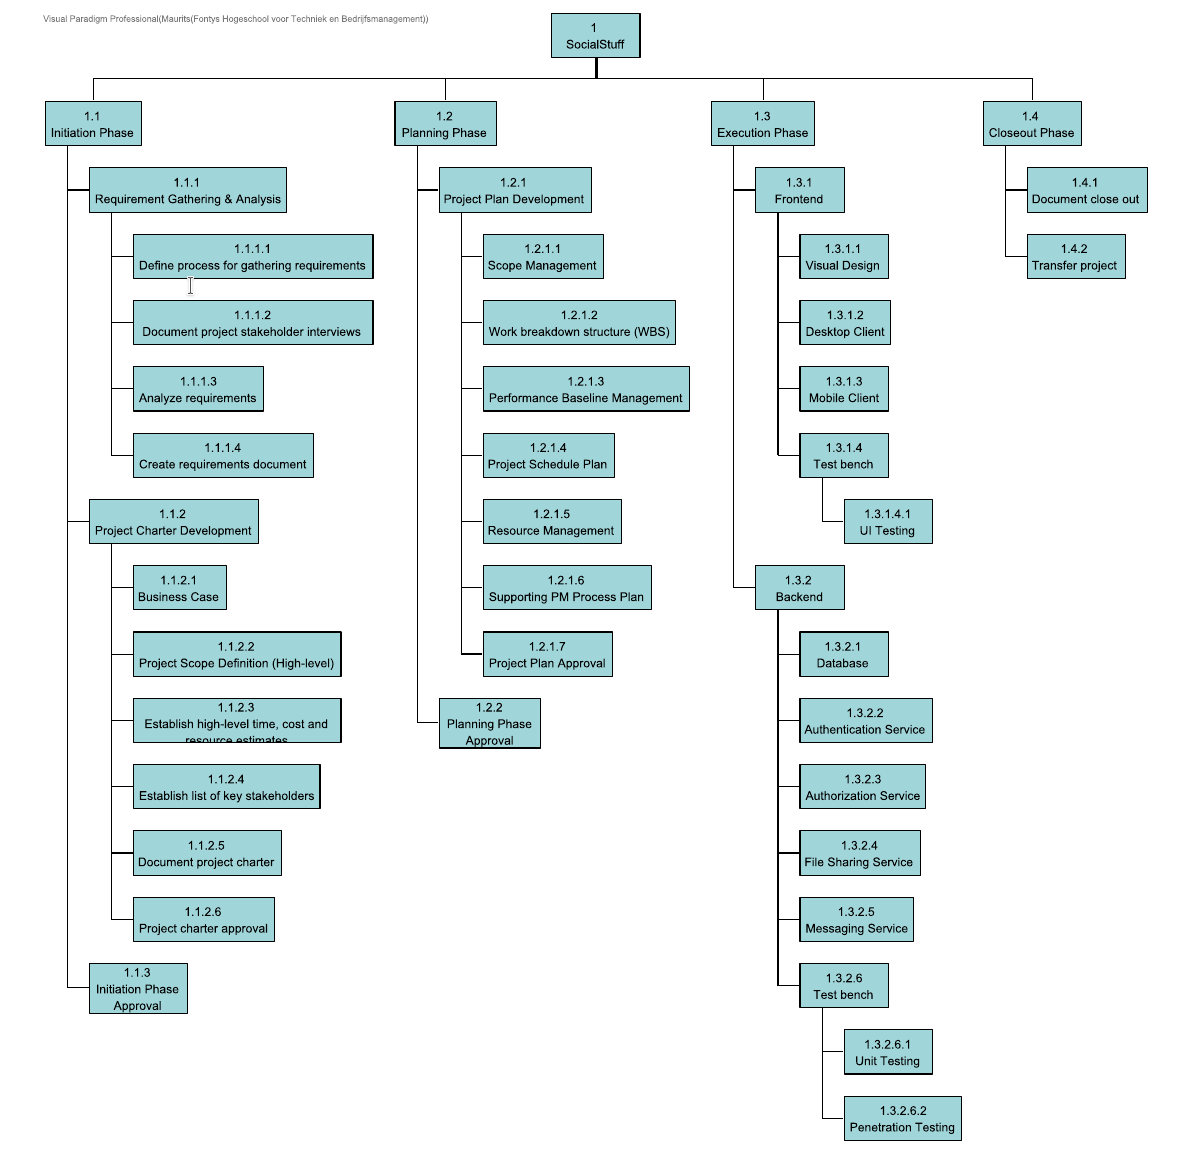
\includegraphics[width=1.0\textwidth]{./images/wbs}
    \caption{Work breakdown structure}
    \label{fig:figure40}
\end{figure}
